% \clearemptydoublepage
% \setcounter{figure}{0}
% \setcounter{tableEng}{0}
% \setcounter{algocf}{0}
% \chapter{基于网格自适应细分的几何与纹理优化}


\chaptera{基于网格自适应细分的几何与纹理优化}
\section{引言}

由于消费级深度相机的广泛普及,3D场景的重建得到了极大的关注。借助于深度相机人们能够很容易的对真实世界的场景进行建模得到场景和物体的三维模型,基于深度(RGB-D)相机的静态场景\upcite{RichardNewcombe2011KinectFusionRD,ThomasWhelan2012KintinuousSE,ThomasWhelan2015ElasticFusionDS,SungjoonChoi2015RobustRO,VictorAdrianPrisacariu2017InfiniTAMVA,AngelaDai2016BundleFusionRG}和动态场景重建\upcite{newcombe2015dynamicfusion,innmann2016volumedeform,yu2017bodyfusion,yu2018doublefusion,xu2019unstructuredfusion,su2020robustfusion,slavcheva2017killingfusion,gao2019surfelwarp,dou2016fusion4d}技术也发生了前所未有的进步。然而,三维重建结果无法满足虚拟现实、混合现实、动画、影视、游戏等领域的需求,一方面是重建几何模型存在瑕疵;另一方面,即使几何模型结果满足基本需求模型外观也无法达到与照片相媲美的程度,很难使人满意也无法直接应用。\par

要获得高保真的纹理映射模型,需要满足两个标准:精确的重建模型和清晰且全局一致的纹理。然而,实际应用中这两个标准常常受到以下因素的干扰。首先,深度相机采集的深度并非绝对准确,当测量距离大于一定阈值时会存在大量误差,并且室内光源的影响也会增加测量误差。其次,在几何模型的三维重建过程中,现有算法为了抵御噪声会使用加权平均方法,这会抹去几何模型的高频细节,使得重建模型整体较为完美但在细节处存在瑕疵。最后,多种误差因素相互叠加,即使采用回环矫正、位姿图优化等算法,相机位姿也只能保证相对准确。这些因素综合影响了图像和几何模型的准确对齐,获取高质量、高保真的纹理映射就需要做进一步的优化。\par


先前的工作采用各种方法试图解决以上所述问题,一般通过合成纹理图像\upcite{bi2017patch}、矫正相机位姿\upcite{zhou2014color}或者细分网格顶点\upcite{ChengleiWu2014RealtimeSR}方面,生成更高质量的三维模型。有的工作不止着眼于单个组件的优化,在先前工作基础上额外提出优化策略使得纹理映射结果更加逼真。如G2Tex\upcite{fu2018texture}采用在基于面投影方法上额外使用从全局到局部的相机位姿矫正方案,成功消除了纹理边界处的大量细缝,生成照片级纹理图像取得了良好的效果。Seamless\upcite{fu2021seamless}也采用面投影方式,并额外采用块合成的方法在纹理边界处重新合成图案以消除纹理。大部分工作聚焦于如何改进或者生成纹理图像以弥补重建模型的误差,但是补偿能力有限,并且只适用于重建模型误差较小情况,未考虑纹理、相机位姿、几何模型之间的耦合性关系,在优化场景的选择上有限制。Intrinsic3D\upcite{RobertMaier2017Intrinsic3DH3}是首个基于明暗变化恢复形状(Shape From Shading,SFS)方法,对场景中的模型形状、模型颜色、相机位姿以及场景光照进行联合优化,但是由于SFS方案会产生纹理复制现象制约了Intrinsic3D方法的应用。最近Fu等人提出JointTG\upcite{YanpingFu2020JointTA}方案对几何、相机位姿、纹理分别进行迭代优化,再采用分层方案代替混合优化策略成功解决Intrinsic3D纹理复制问题并且速度更快。然而,该方案的复杂框架针对不同的优化方案和目标函数进行分别设计,因此在可扩展性和健壮性方面存在一定的挑战,特别是在重建误差较大的情况下。\par

受可微分渲染在三维单视图模型重建\upcite{liu2020general,ShichenLiu2019SoftRA}中的成功启发,本文
提出了一个基于可微分渲染的联合优化深度学习框架,用于同时优化相机位姿、纹理和几何模型。克服现有只对一个因素进行优化而难以达到全局最优解的障碍,并最终得到带有清晰的纹理与精细几何细节的三维重建结果。该框架的核心是一个可微分渲染模块,该模块需要共同参与纹理模型渲染至图像的几何模型、纹理和相机位姿,因此梯度可以在各个组件之间进行传递更新。该框架使用共同的图像间损失函数来优化不同的组件,并具有较高的可扩展性和灵活性。此外,为了突出恢复模型的高频细节,本文还引入了自适应质心细分方法,即仅在纹理丰富区域细分几何模型,以优化几何模型的细节。为了加快模型的收敛速度和优化效果,本文提出了一个交替优化方案,该方案采用分层迭代更新每个组件,从而提高模块的灵活性和训练过程的稳定性。最终,本文成功重建了带有清晰纹理和精细几何细节的三维模型。\par

本文的实验表明,与最先进的方法相比,本文的联合优化框架相比于最新纹理优化方法在真实数据上的可视化结果表现优异。展示了本文在恢复出三维重建模型高频几何细节和表面纹理方面具有优势。\par
总的来说,本章主要包括以下几个贡献:\par
\begin{enumerate}[label=(\arabic*),leftmargin=\parindent,align=left,labelwidth=\parindent,labelsep=0pt]
\item 本文提出了一种基于可微分渲染的全新联合优化方案,将几何模型、纹理图像和相机位姿统一放置于同一框架内,对每个组件分别进行交替优化,最终实现高质量的三维几何模型和高保真的纹理图像。
\item 本文采用对抗生成网络以增强纹理图像的真实感。此外,设计的渲染模块可以灵活嵌入到神经网络中,并且可以自由选择网络结构和优化方式,使整个系统具有高度的可扩展性。
\item 在网格顶点的优化过程中,本文提出了一种自适应细分方法,该方法仅在纹理丰富区域进行细分,可以有效减少计算代价,同时实现与全局细分相同的效果。
\end{enumerate}

\section{算法流程}
\begin{figure}[!t]
    \centering
    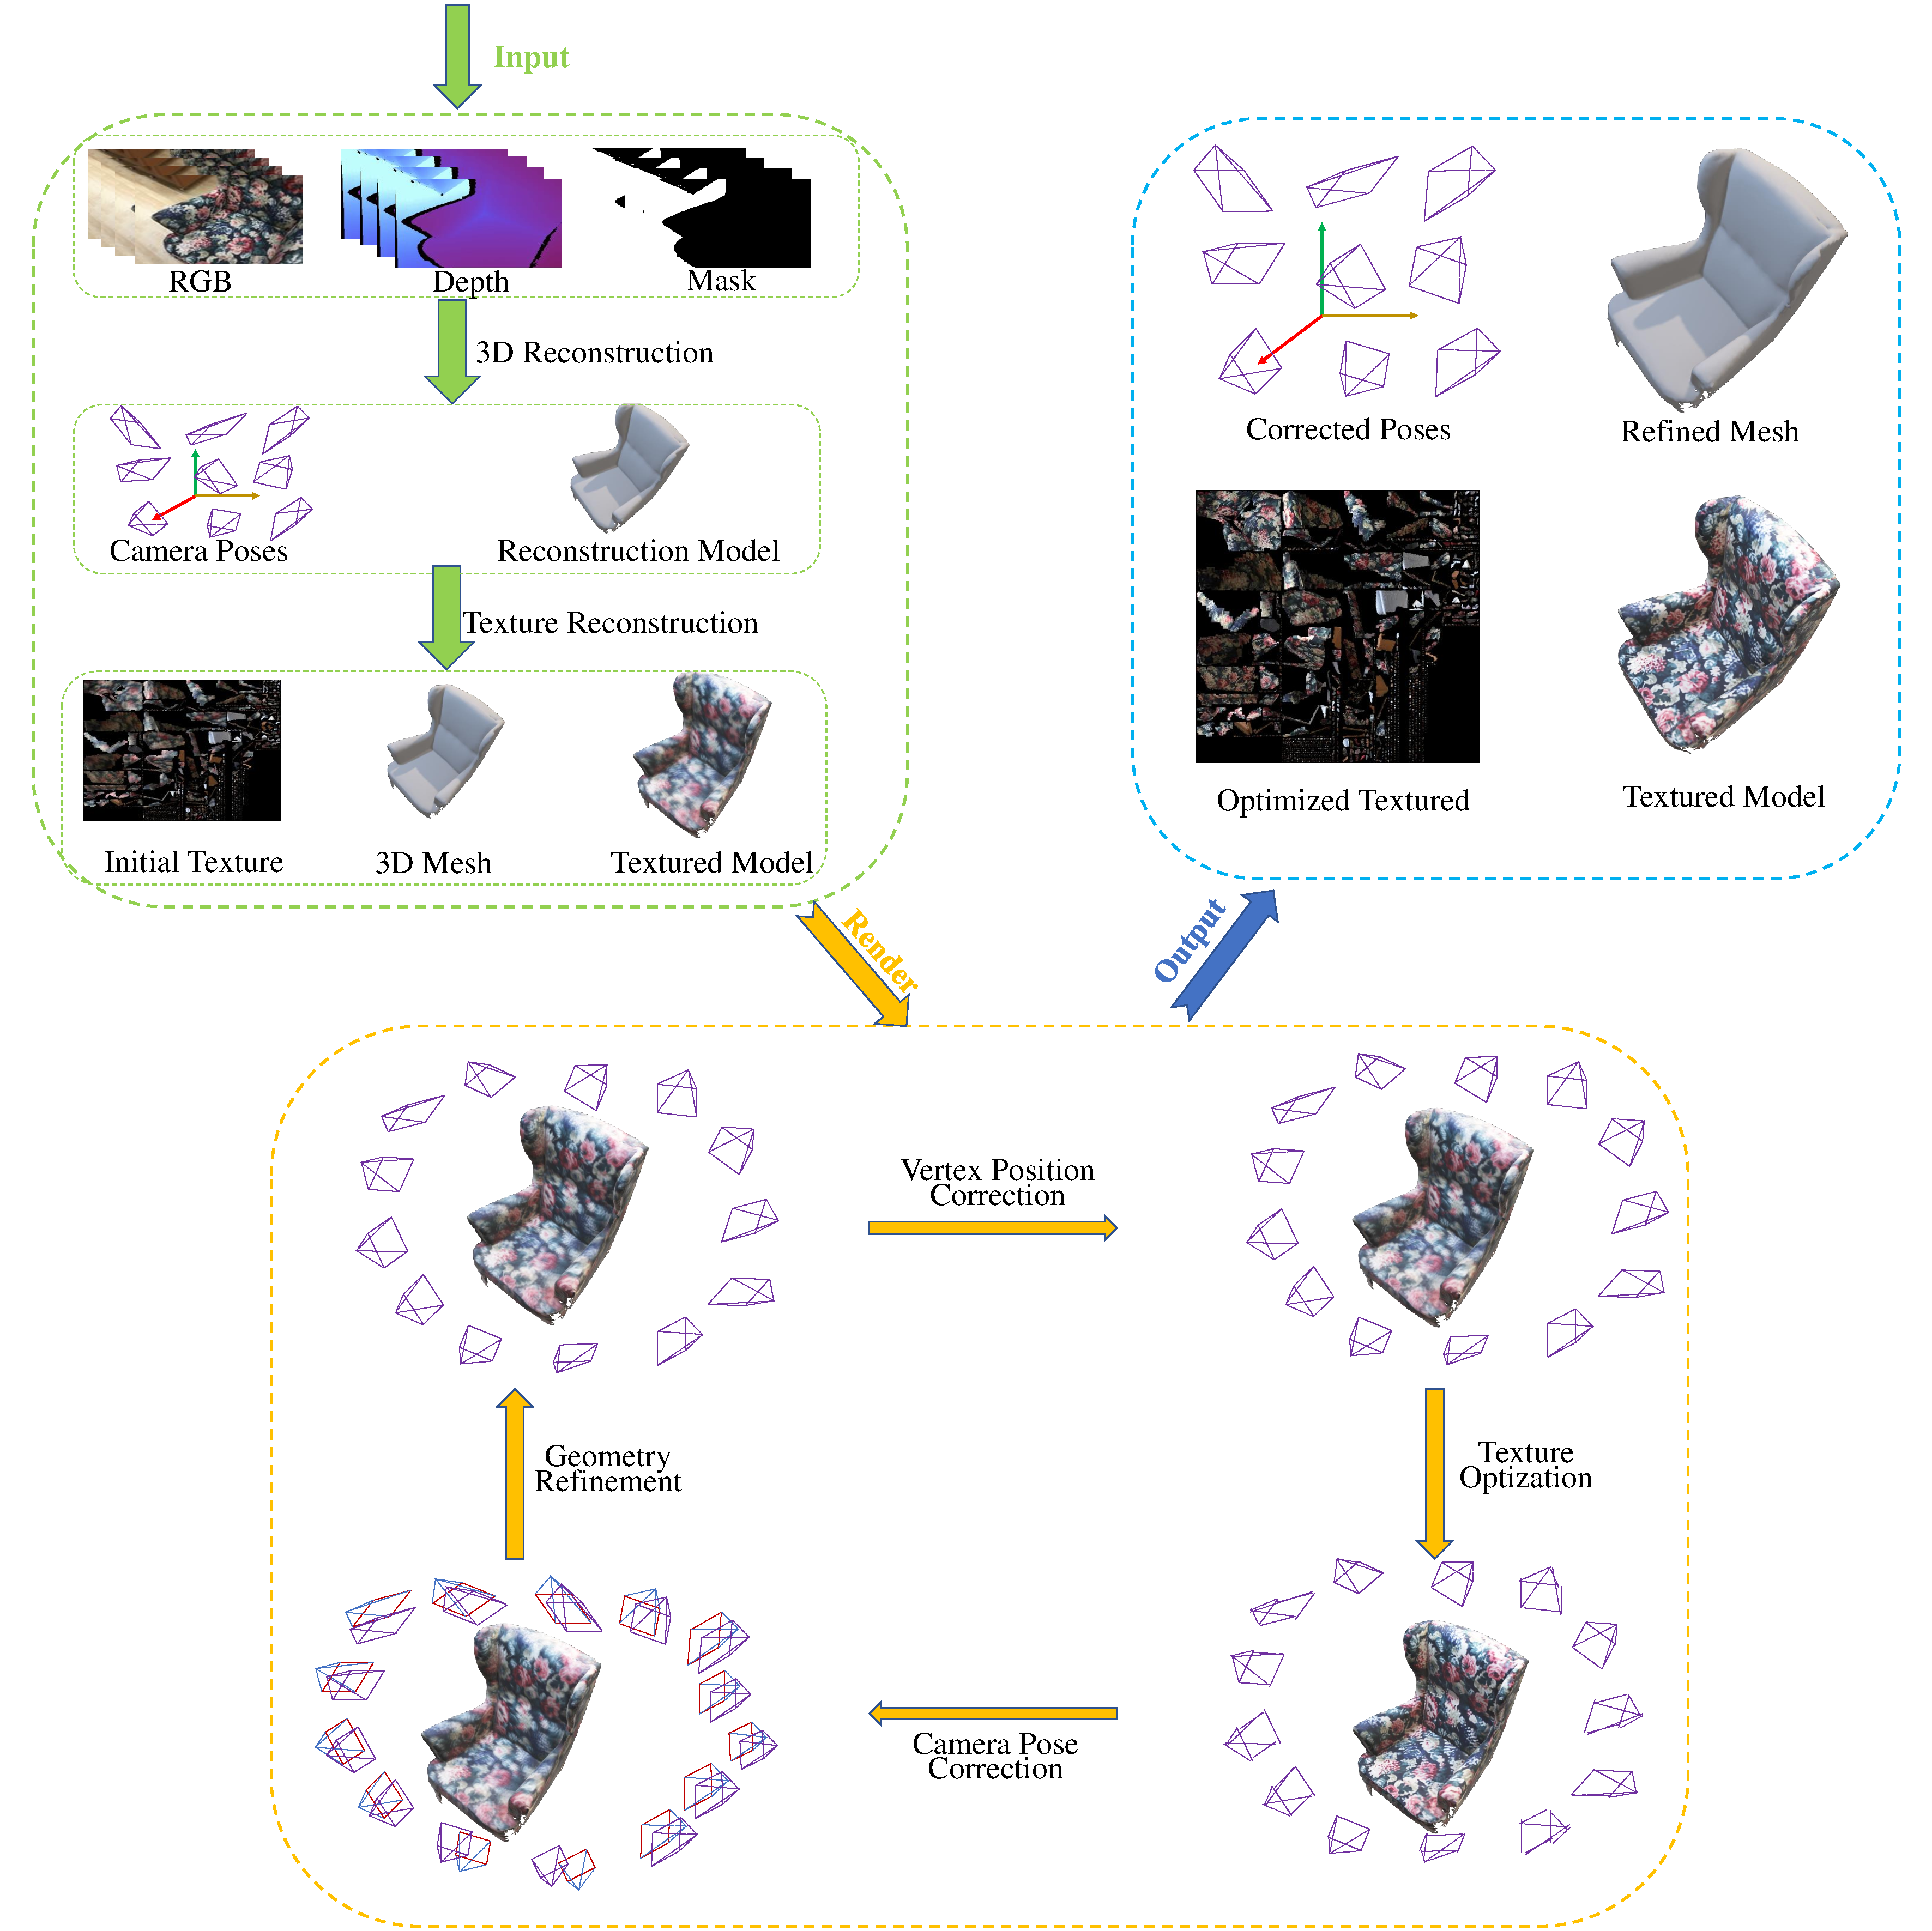
\includegraphics[width=1\columnwidth]{pic/work2/work2.pdf}
    \bicaption{基于可微分渲染的联合优化概述}{The overview of Joint optimization  based on differentiable rendering} 
    \label{fig:work2}
\end{figure}

本文提出的方法旨在利用RGB-D相机获取带有精细几何细节和高保真纹理贴图的三维模型,并通过联合优化算法实现此目标。具体而言,本文通过优化几何模型、纹理图像和相机位姿来实现其重建。优化几何模型可以恢复模型中高频的几何细节,而优化纹理则可以重新生成高保真度的纹理,并通过优化相机位姿来矫正估计不准确的相机位姿。图~\ref{fig:work2}展示了本文算法的完整流程。算法输入包括彩色图像、深度图像和掩码图像,通过三维重建产生初始的三维模型和每个图像对应的相机位姿。然后,利用纹理重建算法生成初始的纹理图像,但由于各种误差存在,初始纹理通常比较模糊。接下来,借助可微分渲染技术,本文矫正相机位姿的不精确性,并利用自适应细分方法在模型中增加几何细节,以及更新其位置以矫正几何误差,最后利用对抗生成网络重合成纹理图像。经过多次迭代优化,最终可以得到具有高频几何细节和优化后的纹理图像的三维模型。\par

在这个部分,本文将详细阐述本文提出方法的具体步骤。本文采用$P$表示纹理图,$M$表示初始几何模型(采用网格表示),$T$表示相机外参,$K$表示相机内参。其中,$I_c$、$I_D$和$I_S$分别表示手持RGB-D相机拍摄的彩色图、纹理图以及采用标准计算机图形学管线生成的掩码图。纹理、几何模型和相机位姿是本文目标恢复清晰保真纹理的关键,且三者之间耦合性极高。值得注意的是,渲染本身就需要纹理、相机和几何模型的共同参与,这与本文的优化目标高度契合。借助pytorch3d\upcite{ravi2020pytorch3d}可微分渲染框架,本文可以依据其渲染流程制定更加合理的优化策略,即分别对每个部分进行交替迭代优化而非采用多变量共同优化的混合策略,可以使得纹理、相机位姿和网格的优化过程相对独立,但是又高度内聚。下一个章节中,本文将详细介绍在优化框架中,纹理、相机位姿和网格的各自优化过程。\par


\subsection{数据预处理}
本文的算法可以是深度相机采集的原始数据,但是为了保证输入数据的规范性以及符合优化算法的输入,原始数据还需经过预处理,本文仍旧采用第三章第四节所述预处理方法。由于在网格重建后往往会有重复顶点,三角形面片可能会自相交,不符合网格的2D拓扑流形结构,在移动顶点位置后会发生显而易见的的裂缝。此外,由于在重建过程遮挡,噪声干扰等因素使得重建模型存在明显的孔洞。为了防止优化过程出现异常情况,如裂缝现象。本文先用meshlab\upcite{LocalChapterEvents:ItalChap:ItalianChapConf2008:129-136}剔除重复顶点和面片以及零面积面片,以保证几何模型的规范性。


\subsection{相机参数优化}
在基于RGB-D的三维重建中,通常使用光束平差法\upcite{BA}估计初始的相机位姿,然而估计结果只能保证相对准确,使用不完美的相机位姿渲染图像会导致渲染图像和采集图像错位。为了解决这个问题,本文利用可微分渲染框架对相机位姿进行矫正。在第三章中介绍的相机优化方法的基础上,本文额外增加了一个变形场$F$,用于矫正相机内参。为每个图像添加一个非刚性的优化过程,以矫正因不精确的几何和光学畸变而导致的复杂扭曲。设图像平面$I_i$上一点$\mathbf{u}$,定义在图像$I_i$上的变形函数$F_i$,$f_{i,l}$为二维向量。则变形函数定义为:
\begin{equation}
	\mathbf{F}_{i}(\mathbf{u})=\mathbf{u}+\sum_{l} \theta_{l}(\mathbf{u}) \mathbf{f}_{i, l}
\end{equation}
其中,$\theta_{l}(\mathbf{u})$为双线性插值函数,考虑到在给投影顶点施加移动向量,投影位置会在像素点之间,所以本文应用双线性插值函数为投影选择最佳的合适位置。由于投影过程与矫正过程是可微的,相机内外参矫正可以有机地结合。\par
受三维重建算法\upcite{DejanAzinovic2021NeuralRS}启发,本文使用6层Relu\upcite{agarap2018deep}激活函数的多层感知机在像素空间内附加二维变形场,以考虑输入图像中可能的扭曲或相机固有参数的不准确性。本文实验研究后发现,在同一场景中,所有图像扭曲失真情况的原因相同,如可能来自于相机内参的不准确性。在矫正域每一帧共享多层感知机的参数。在优化过程中,相机光线首先使用在使相机位姿投影至图像平面上然后从变形场检索的2D向量,然后用重投影误差函数公式\eqref{pose},共同优化变形场和相机位姿。

\subsection{基于自适应细分的网格优化}
\begin{figure}[ht]
    \centering

    \includegraphics[width=1.0\columnwidth]{pic/work2/mesh.pdf}
    \bicaption{基于可微分渲染的几何模型优化概述}{Overview of geometric model optimization based on differentiable rendering}
    \label{fig:mesh}
\end{figure}


仅仅优化相机参数不足以保证网格上任意顶点投影至每个视角得到一致颜色,尤其是在网格重建误差较大情况下。此外,在重建三维模型时一般会选用加权平均方法来抵抗重建过程中的噪声,虽然这种方法卓有成效,但是会造成过平滑的效果致使网格失去几何高频细节。本文同样也借助于可微分渲染方法恢复出几何表面的高频几何细节。本文为网格上每个顶点施加偏移量来矫正几何误差。\par
仅仅只更新顶点位置不足以保证几何模型细节突出,因为几何模型本身就过于平滑。本文采用质心细分网格方法增加三角形面片数目,一方面能使得模型更加契合真实世界场景,另一方面能减小顶点优化时发生漂移现象。即使如此,细分网格代价是巨大的,增加顶点面片数目会线性增加渲染时间,并且在一些含有平面较多且纹理单一的几何模型上细分视觉效果并不明显。本文实验中发现优化几何模型时,顶点移动频繁发生在纹理丰富的地方,而纹理较为单一时顶点移动并不明显。因此本文建议根据场景本身的纹理丰富程度来决定是否要细分以及细分的程度。如图~\ref{fig:subdivion}所示网格自适应细分流程。具体地,本文遵循以下步骤:
\begin{enumerate}[label=(\arabic*),leftmargin=\parindent,align=left,labelwidth=\parindent,labelsep=0pt]
	\item 用soble算子提取所有视角的梯度图$\nabla g_i$,作为细分面片的依据。
	\item 计算几何模型上每个面片$f_j$投影至每个可见视口$i$的面积$A_{ij}$,并求出面积总和$\sum_{i}^{n} A_{ij}$。
	\item 计算每个面片$f_j$采样概率$\sum_{i}^{n} A_{j} / \sum_{j}^{m}\sum_{i}^{n} A_{ij}$,其中m为几何模型中面片数量,n为视角数量。
	\item 按照概率对所有面片进行无放回随机抽样,并设定采样概率阈值为0.5,在阈值概率之上面片才会被选取。
	\item 对所选择面片$f_j$进行质心细分。
\end{enumerate}

\begin{figure}[ht]
    \centering
%  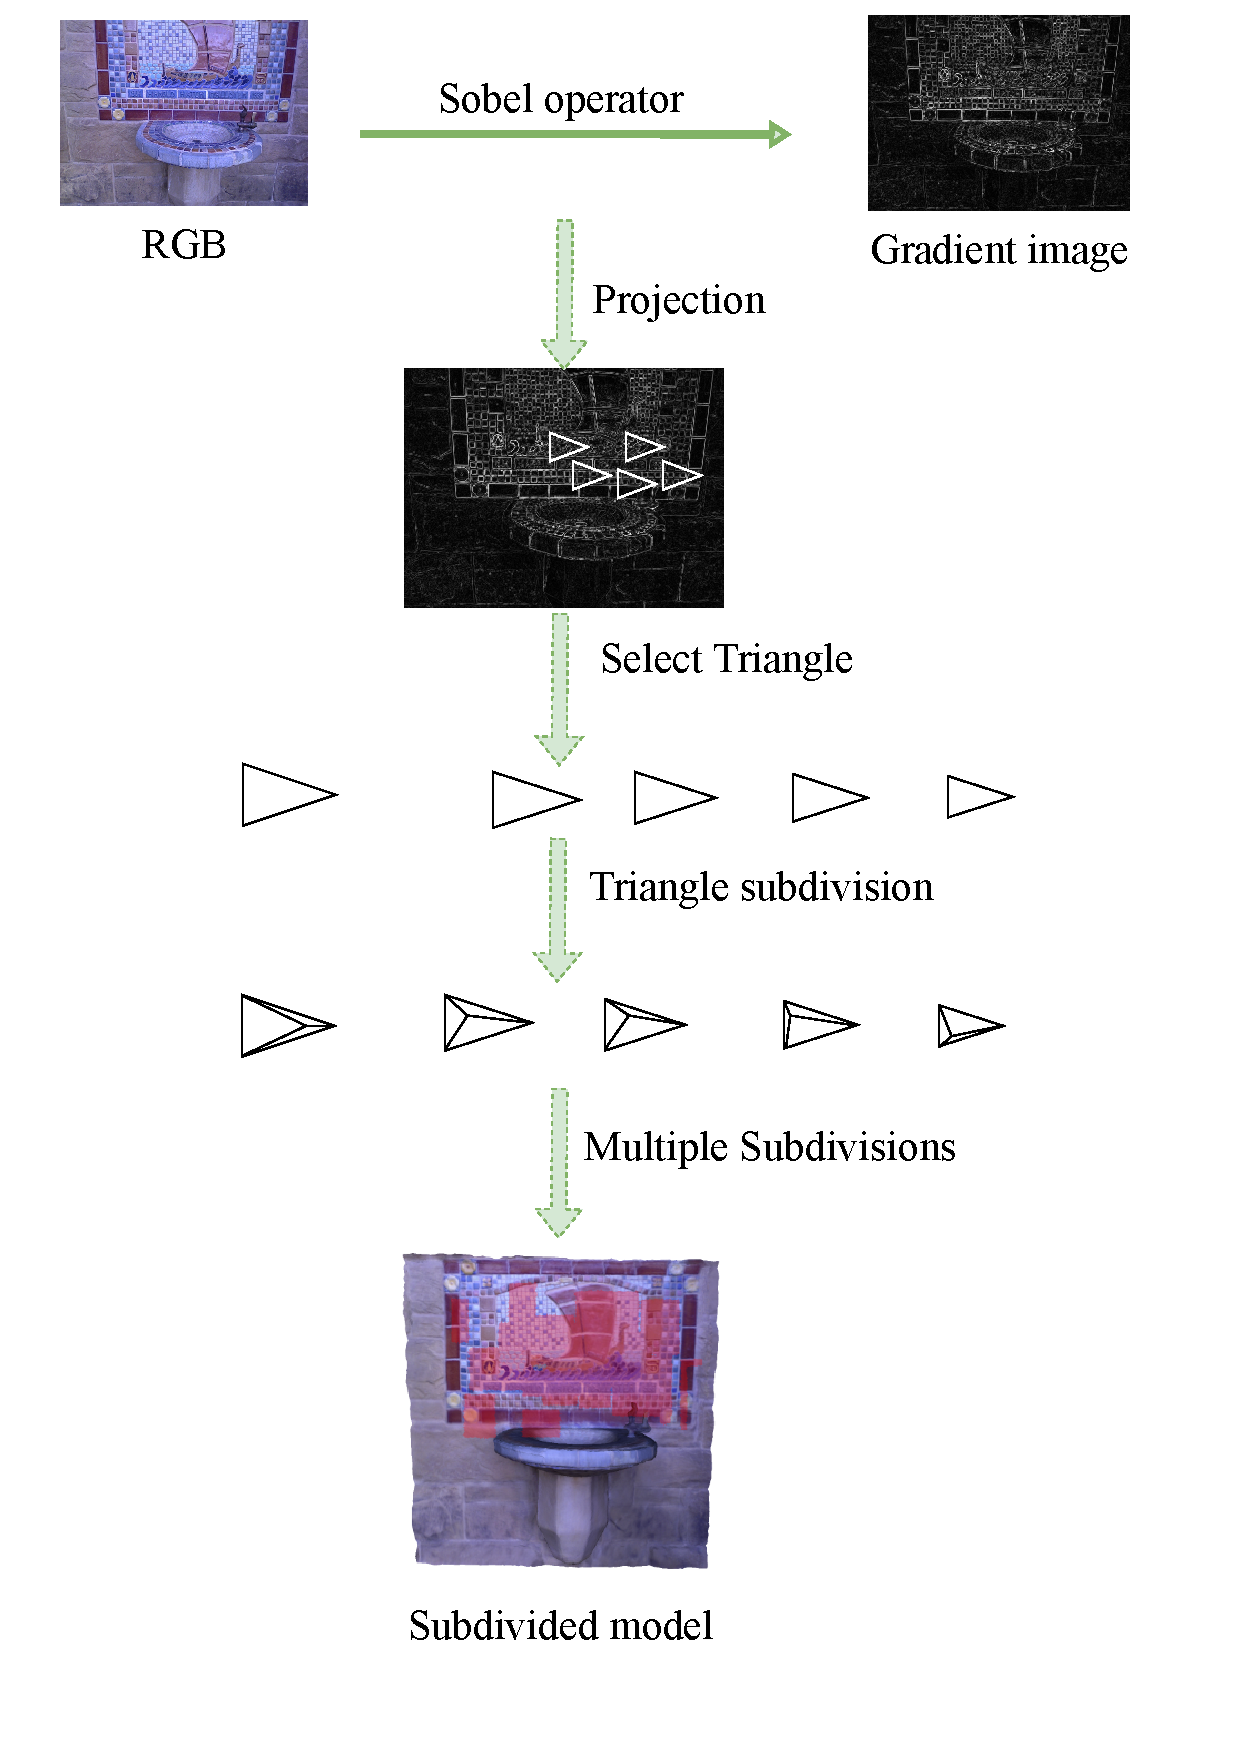
\includegraphics[height=0.5\textheight,keepaspectratio]{pic/work2/Mesh_subdiv.pdf}
    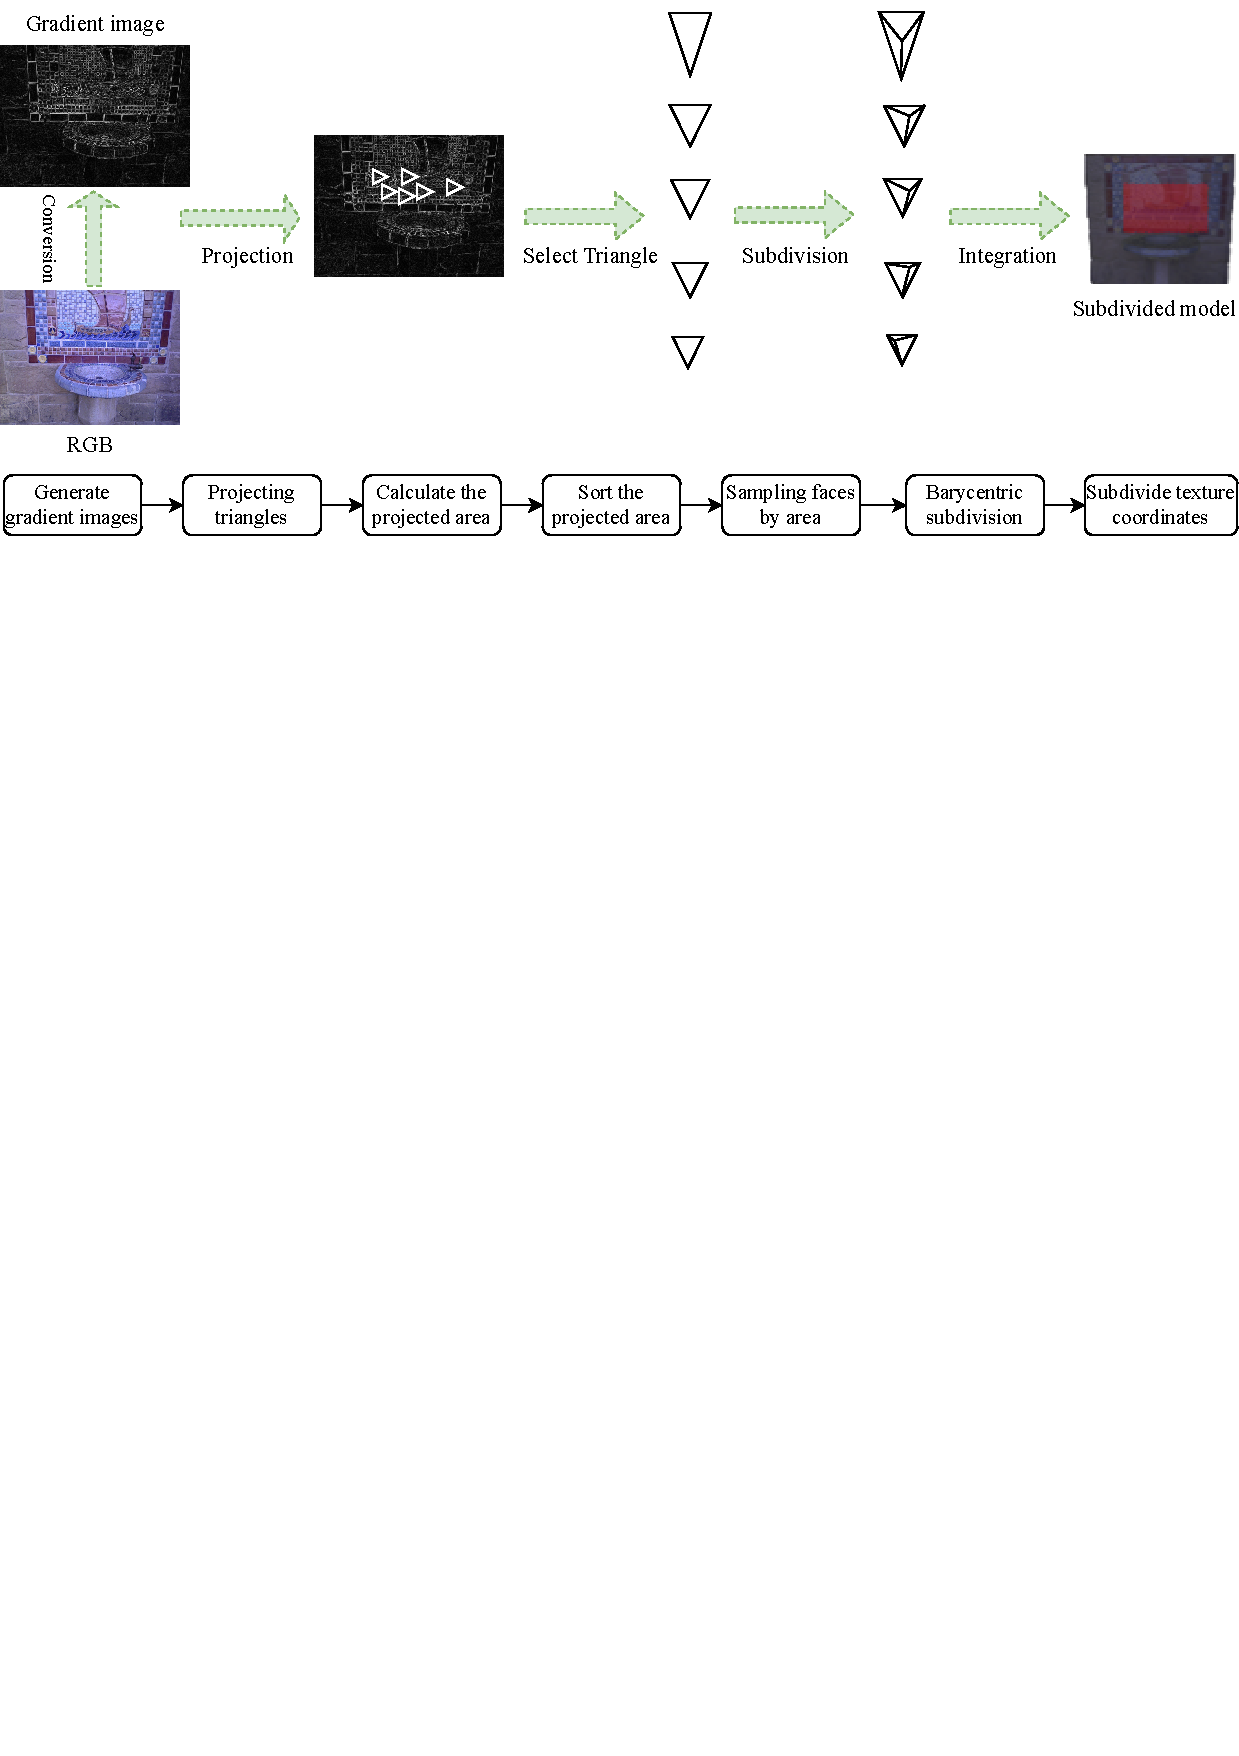
\includegraphics[width=1.0\columnwidth]{pic/work2/mesh_subdivision.pdf}

    
    \bicaption{网格自适应细分概述}{Overview of Adaptive Mesh subdivision }
    \label{fig:subdivion}
\end{figure}

本文在第四步随机抽样时,为了防止太多的面片不在查询集合中,本文使用中位数而不是平均值作为采样阈值。细分完成后,本文仍用同样的方式增加对应的纹理坐标,以保持顶点和纹理坐标的对应关系。\par
优化几何模型时仅仅有图像间损失是远远不够的,因为每次迭代中顶点移动不受约束,会破坏网格模型的拓扑结构,导致三角形退化。因此本文在图像损失基础上增加了几何正则化项,即拉普拉斯项、法线一致性项和$L2$ 范数。\par
拉普拉斯项定义为顶点坐标减去其临近顶点的加权和,在优化过程中可以保持局部几何特征不变。在优化过程中,拉普拉斯损失项可以帮助模型收敛到一个更加平滑的解,从而提高几何模型优化的准确度和稳定性。它也可以有效抑制因噪声或不规则采样而产生的噪点,使得优化结果更加符合实际。令$V \in \mathbb{R}^{n\times3}$为存储顶点位置的矩阵,则拉普拉斯项定义为:
\begin{equation}
	E_l = \sum_{i=1}^{n}\left \| LV \right \|_2 
\end{equation}
其中,$L\in\mathbb{R}^{n\times n} $是网格的拉普拉斯图。\par
在优化过程中为了防止顶点偏移初始位置太远,本文用$L_2$正则化项来约束顶点偏移量。其中$\mathbf{v}_{i}$为初始网格的顶点坐标,$\widetilde{\mathbf{v}}_{i}$为当前网格顶点的坐标。
\begin{equation}
	E_{r}=\sum_{i}^{n}\left\|\mathbf{v}_{i}-\widetilde{\mathbf{v}}_{i}\right\|^{2}
\end{equation}

最后,为了保证网格具有平滑性,本文额外使用了网格法线一致性损失。即利用余弦相似度计算相邻面片的法线一致性。
\begin{equation}
	E_n= \frac{1}{|\overline{\mathcal{F}}|} \sum_{(i, j) \in \overline{\mathcal{F}}}\left(1-\mathbf{n}_{i} \cdot \mathbf{n}_{j}\right)^{2}
\end{equation}
其中,$\overline{\mathcal{F}}$代表共享一条边的相邻三角形面片的集合。$i$,$j$表示任意一对儿三角形面片。\par
最终网格重建损失项表示如下:
\begin{equation}
	L_M = L_T + \lambda_l E_l +\lambda_r E_r+\lambda_n E_n
\end{equation}
在实际优化中,本文分别设置$\lambda_l = 1000$,$\lambda_r = 1000$,$\lambda_n = 10$。\par

详细更新流程如图~\ref{fig:mesh}所示,对于重建模型本文首先进行自适应细分策略,然后经过可微分的光栅化阶段,从Zbuff中获取深度图和掩码图像。然后本文用布林冯着色模型\upcite{blinn1977models}对投影像素着色得到渲染图像,最后损失项回传梯度,更新网格顶点位置。

\subsection{纹理重合成}
仅仅只矫正相机位姿和网格顶点位置是不够的,优化结果并不能完全消除噪声。况且本文采用顶点加权融合方式生成纹理,仍存在模糊并且缺失细节。对于残留的微小位姿误差、几何误差、光源干扰等再使用优化算法收效甚微。受纹理图像合成法\upcite{bi2017patch,JingweiHuang2020AdversarialTO}的影响,本文利用图像合成法合成新的纹理图。具体算法与第三章所著的纹理合成模型相同。本文在此基础上额外添加了频域空间损失以保证纹理合成不会出现模糊失真。\par

在生成对抗网络中尽管合成图像已经足够逼真,但是真实图像和生成图像在空间域中仍旧存在不易察觉的差距。将图像变换至频域后,这种差距变得尤为明显。基于这种发现,Jiang等人\upcite{jiang2021focal}提出新的频域损失,减少图像间的频域差距。本文由此得到启发,在对抗生成网络中加入频域损失函数。它可以自适应的关注深度生成模型难以合成的频率分量,纠正对神经网络存在的偏差性。从而提升模型在图像空间域合成的微小细节的能力。文本在公式\eqref{texture}基础上本文额外添加了Focal Loss损失:
\begin{equation}
	L_\mathrm{FFL}=\frac{1}{M N} \sum_{u=0}^{M-1} \sum_{v=0}^{N-1} w(u, v)\left|F_{r}(u,v)-F_{f}(u, v)\right|^{2}
\end{equation}
其中,$M,N$为图像宽高,$w(u,v)$为图像$(u,v)$位置处的频域分量权重。\par
经过若干次迭代交替训练判别器$D$和纹理$P$后,神经网络会学习三维场景中存在的各种误差,并在生成容忍这些误差的清晰的纹理图像,而不需要额外更新已有的纹理映射关系。 与加权融合方法生成的纹理相比,优化后的纹理更逼真,更接近真实彩色图像。\par

\subsection{交替优化}
相似于之前工作\upcite{YanpingFu2020JointTA},本文使用联合优化策略优化相机参数、几何模型和纹理。本文用相机-几何模型-纹理优化顺序进行。一方面是在相机和网格优化中纹理生成方法不同于对抗神经网络的像素重生成方法,另一方面在矫正相机参数和网格后,对抗生成网络效果重生成的纹理更加贴近于真实世界场景。具体地,本文采用外部循环方法分别优化参数集合$(T,M,P)$。本文首先固定参数$(M,P)$,通过最小化损失函数$L_T$以优化每一帧的相机参数$T$至$T'$;其次,本文使用参数$(T',P)$最小化损失函数$L_M$优化几何模型$M$至$M'$;最后本文使用并固定前两次的结果参数$(T',M')$最小化对抗损失$L_{adv}$来优化纹理$P$至$P'$。\par
在时间和效率的权衡下本文重复外循环优化策略3次。并且本文遵从由粗到细的策略优化不同的目标。具体地,在每一次外部迭代$t\in \left \{ 1,2,3 \right \}$中本文用指数衰减方式控制内部迭代次数,即内部迭代次数为$\text{epoch}  =\frac{s}{2^{t-1}}$,其中s为每一个内部迭代初始的轮数。此外,学习率也会相应地进行调整。实验研究发现,利用指数衰减策略,可以保证最终效果的同时显著减少优化时间。本文设置初始的优化相机参数、优化几何模型和纹理次数分别为50,50,100。

\section{实验结果与讨论}
在本节中,本文在各种不同的真实场景下进行定性分析,以证明所述方法的有效性。本文与最近提出的纹理优化方案G2Tex\upcite{fu2018texture},JointTG\upcite{YanpingFu2020JointTA}和ATO\upcite{JingweiHuang2020AdversarialTO}进行比较。其中G2Tex为基于面的投影方案生成的场景纹理,面纹理直接来自于投影图像,最终生成的纹理清晰度与拍摄照片一致。这种方案旨在解决相邻面片纹理间的错位现象。ATO、JointTG与本文提出的方法,主要以顶点颜色加权融合生成物体纹理,虽然不会发生纹理图像的错位,但是容易产生模糊伪影等问题。不同的是ATO采用生成对抗网络重新生成新的高清纹理图像,作为纹理映射结果。JointTG通过联合优化方法,同时优化纹理、网格和相机位姿抵抗重建模型过程中的噪声以获取最清晰的纹理。对于另一个联合优化方案Intrinsic3D\upcite{RobertMaier2017Intrinsic3DH3},因为Intrinsic3D在优化过程中,采用细分体素方案生成密集网格作为算法的结果,不需要在算法输入时候提供网格模型。而本文数据集提供了初始的网格模型,为了标准统一,所以不再进行实验对比。
在实验中,使用各个方法发布的源代码进行比较。由于G2Tex与JointTG作者在论文中说明需要选择关键帧作为算法的输入。在某些没有发布关键帧序列的场景下,如椅子数据集\emph{Chairs},本文按照清晰度度量指标选出若干张覆盖物体全景且最清晰的图像为关键帧,作为G2Tex与JointTG算法的输入。最后,本文用消融学习策略证明本文所提出的算法的有效性。本文的实验环境与评估指标等其它实验设置均和第三章所描述的保持一致。


\subsection{公共数据集上结果与分析}
\begin{figure}[!t]
\centering
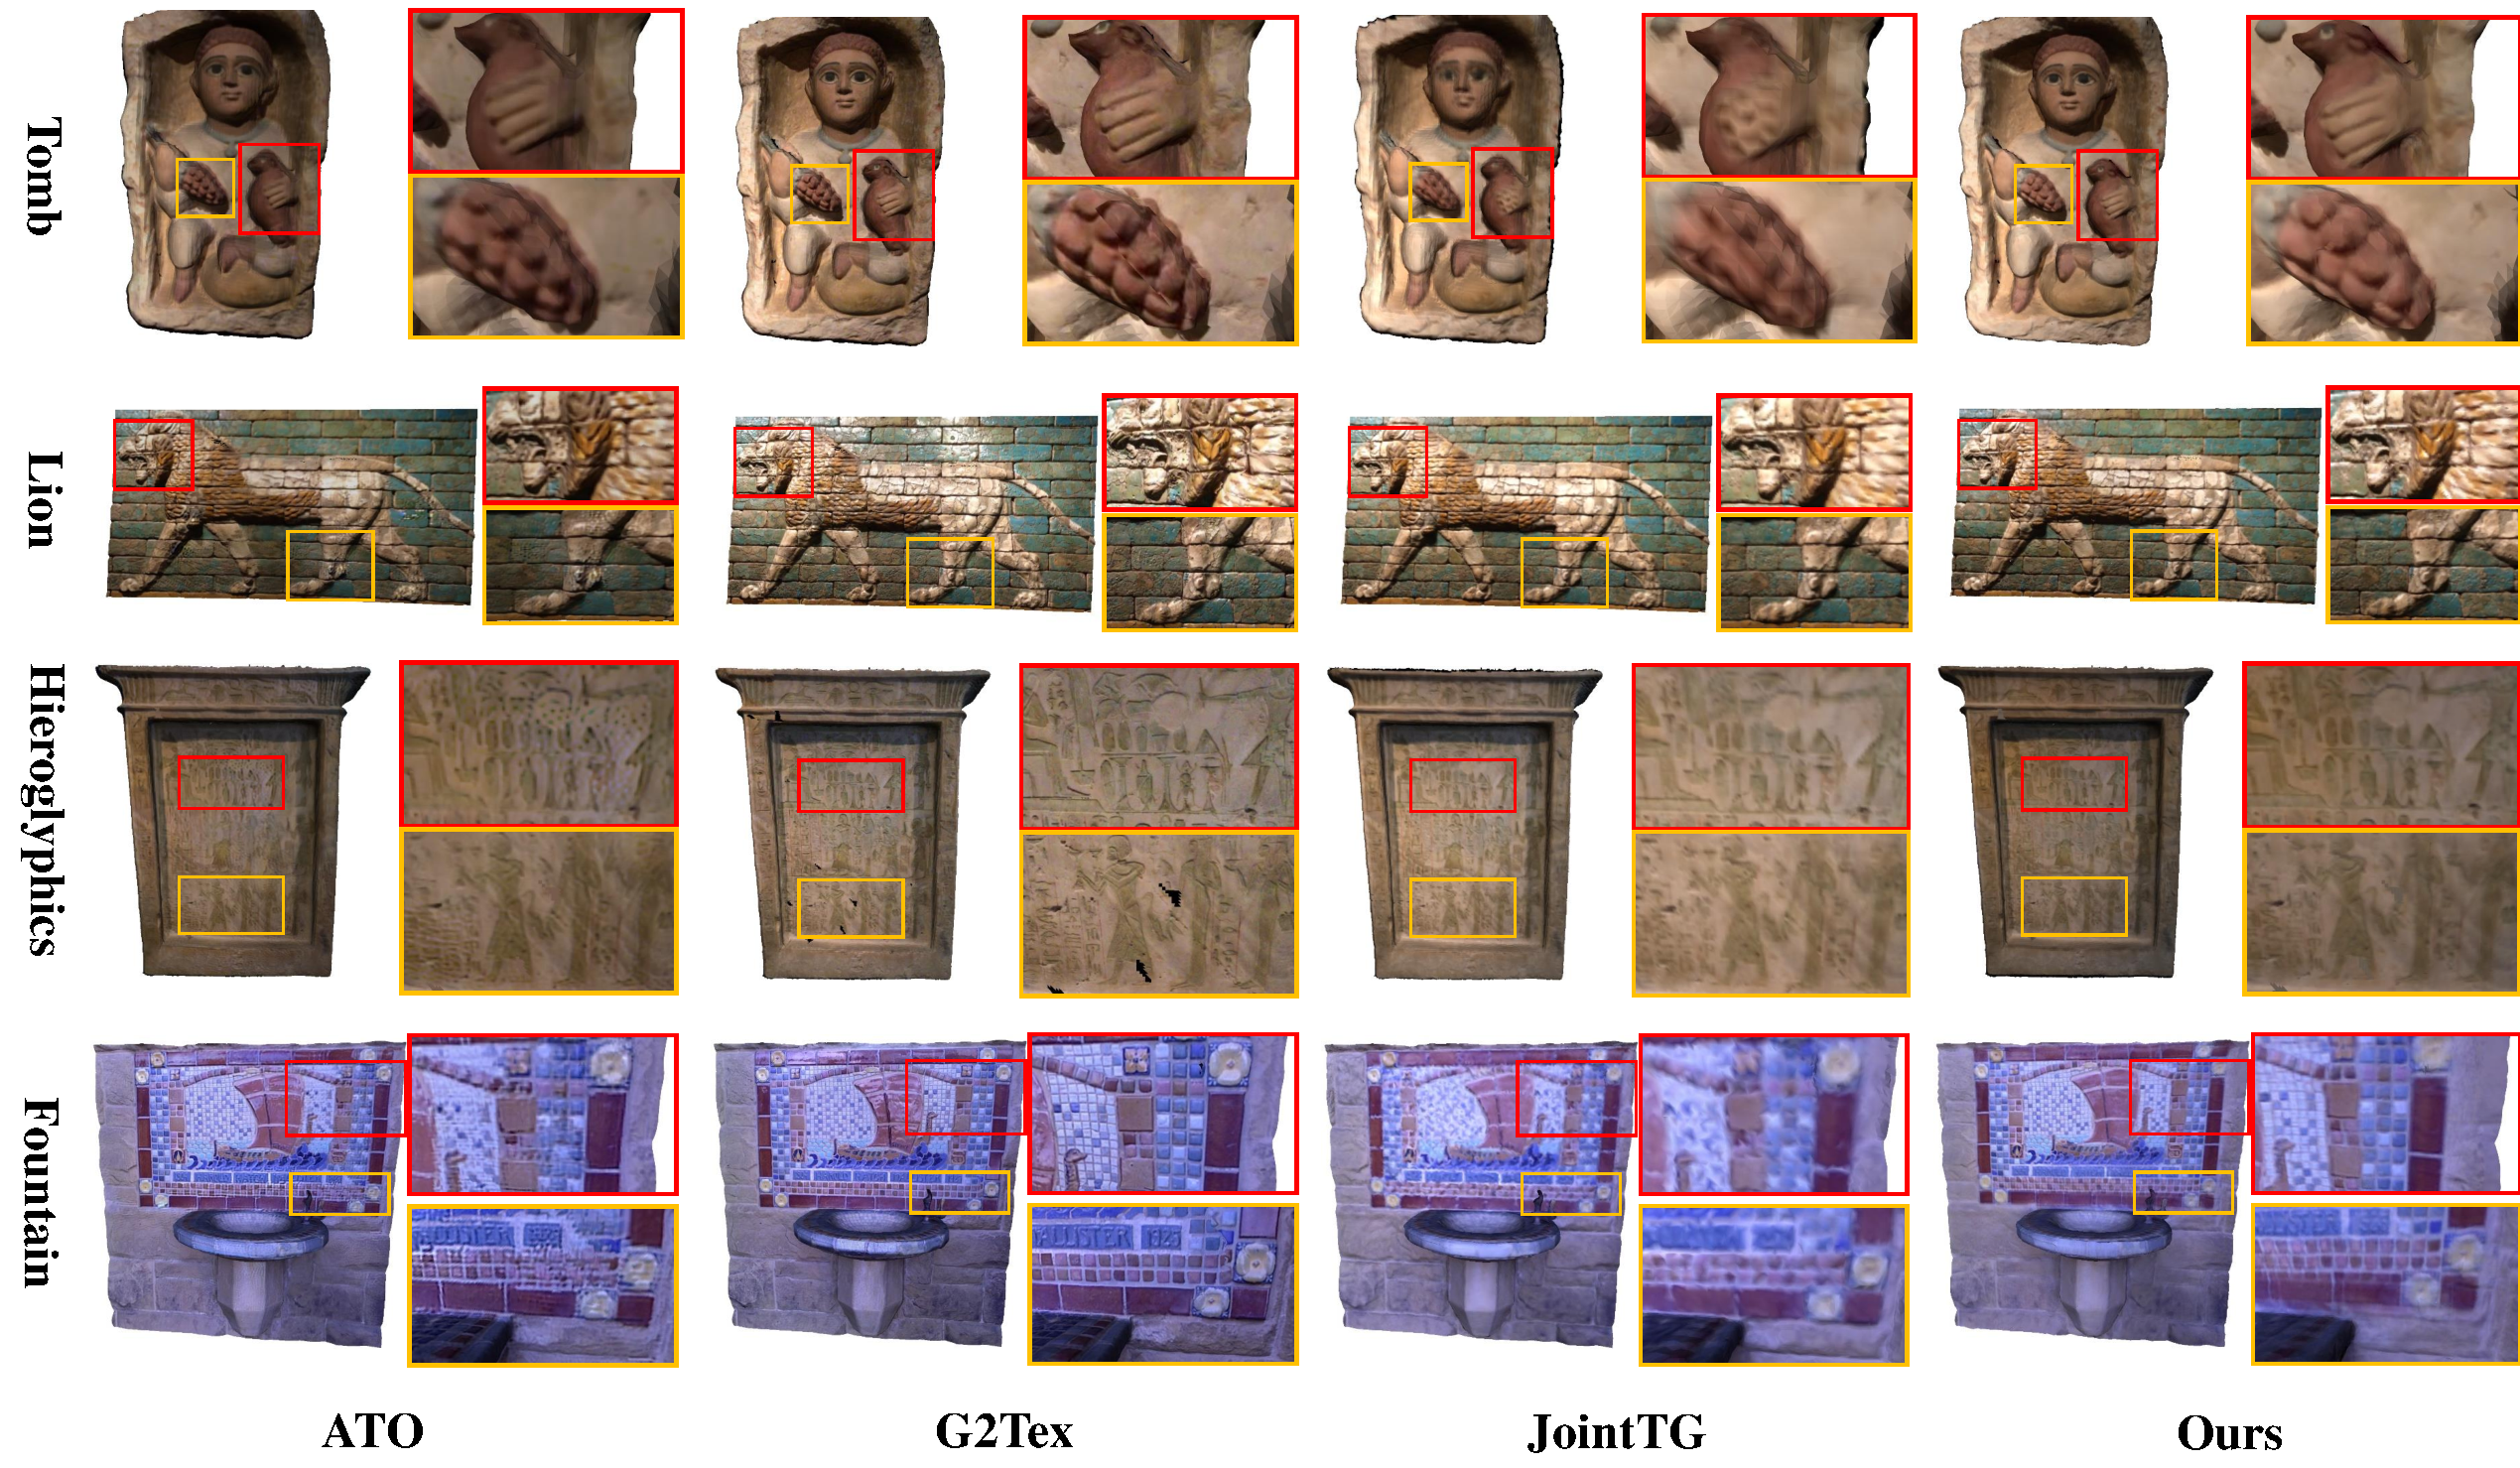
\includegraphics[width=1\linewidth]{pic/work2/compare3.pdf}
\bicaption{公共数据集上不同渲染方法的视觉比较 1}{Visual comparison of different rendering methods on public datasets 1}

\label{fig:ex2_3}
\end{figure}

本文首先在Intrinsic3D发布的公共数据集上进行评估,初始网格模型来自于Intrinsic3D重建出的体素模型。为了便于使用本文用Marching cubes算法\upcite{lorensen1987marching}抽取出基本的三维网格。如图~\ref{fig:ex2_3}所示,图片第一二三行均来自此数据集。该数据集颜色较为单一,且平面场景较多,这为纹理优化带来挑战性。本文的方法可以获取全局一致的纹理效果,从数据集\emph{Tomb}(图片第一行)可以看出本文所提出方法比ATO与JointTG产生的纹理映射结果清晰,从图中红色框展示的鹰的眼睛以及橙色框中的玉米棒图案可以看出。ATO方法虽然能产生全局一致的纹理,但是在某细节出会出现伪影,如\emph{Lion}场景下橙色框所展示的狮子的脚部,\emph{Hieroglyphics}场景下红色框中的图案。由于在平面场景下细节不够丰富,使用生成对抗网络无法完全重建物体的纹理细节,即使能够容忍较小的相机误差和几何误差,但是在局部地方仍然有模糊现象。\emph{JointTG} 在实现场景纹理细节处表现并不完美,如\emph{Hieroglyphics}的图案,\emph{Tomb}中人物的手部等。场景中模型顶点较少,无法突显出场景的局部细节。从清晰度角度看,G2Tex的结果最佳,但是无法保证全局一致性。如图第一二行红色框所示,纹理图像有明显的断裂情况。\emph{Hieroglyphics}场景下会出现孔洞现象。最后,本文也在Zhou等人\upcite{Zhou2018}发布的\emph{Fountain}场景下比较基线方法,该数据集视角非常稀疏。在此数据集上,本文的方法仍然可以获得高保真度的纹理。虽然,G2Tex使用面投影方法能产生最佳纹理,但是在加权融合策略下,本文方法在细节和清晰度方面优于ATO与JointTG。\par

\begin{figure}[!t]
\centering
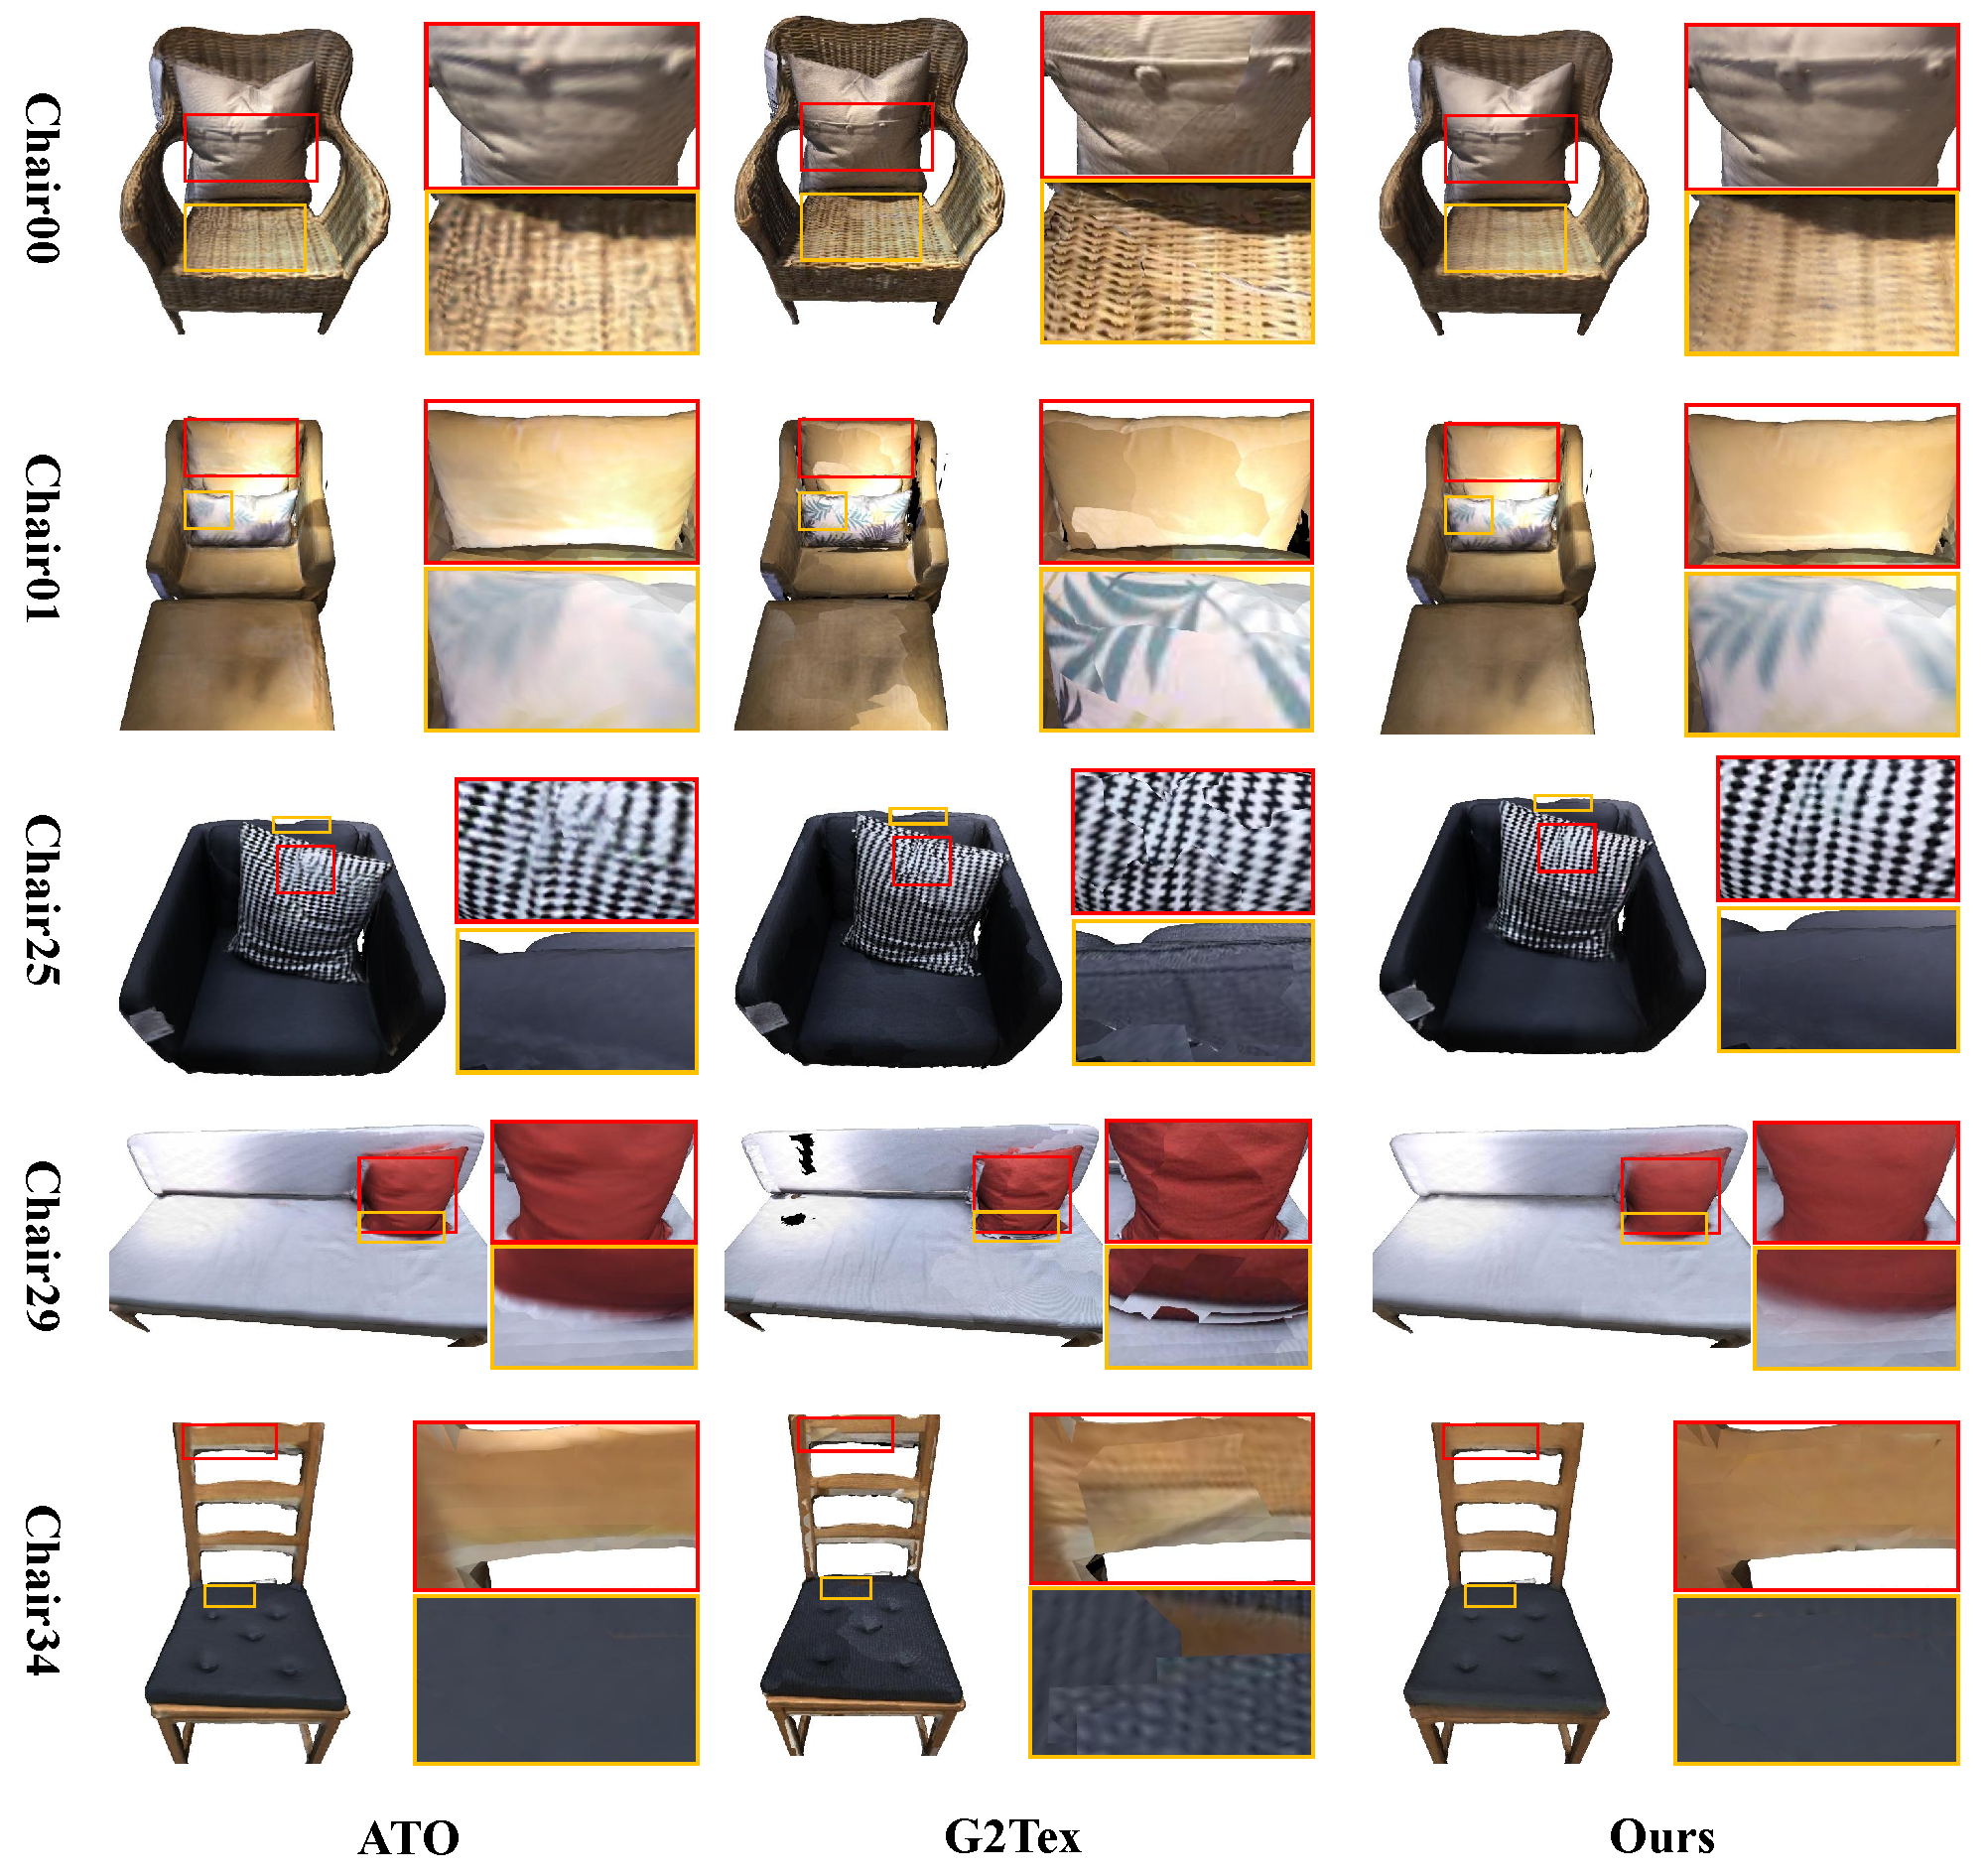
\includegraphics[width=1\linewidth]{pic/work2/compare1.pdf}
\bicaption{公共数据集上不同渲染方法的视觉比较 2}{Visual comparison of different rendering methods on public datasets 2}

\label{fig:ex2_1}
\end{figure}

本文在Chairs数据集同样做了对比,如图~\ref{fig:ex2_1}所示。该场景与Intrinsic3d数据集相比,纹理较为简单,给相机位姿矫正带来了挑战。由于该场景和模型顶点数量较少,JointTG利用顶点颜色表示物体表面外观的方法并不适用,所以本文不做比较。从图中所展示,本文与ATO均可得出全局一致的纹理,而G2Tex的全局矫正和局部扭曲纹理坐标方案并不能完全消除纹理裂缝。从图中\emph{Chair01}、\emph{Chair25}和\emph{chair29}场景下橙色框所展示,纹理图像间有明显的断裂。本文方法在颜色单一的场景下也能保持鲁棒性,而且从\emph{Chair01}场景的橙色框中可以看出,本文能够恢复出比ATO更丰富的纹理细节。\par

最后,本文在G2Tex发布的公共数据集上进行比较,如图~\ref{fig:ex2_2}所示。该场景使用kinect \emph{v}1深度相机拍摄。图像分辨率低,较为模糊,而且场景受灯光,几何噪声等因素干扰较明显。通过定性结果证明,本文的在恢复纹理外观细节方面优于ATO与JointTG。ATO通过融合来自多个视图的纹理信息和使用对抗网络来获得更好的纹理。尽管如此,它还是无法恢复微小细节,如\emph{Bolster1}场景。JointTG生成的纹理和网格在视觉上是和谐的,但是由于在优化网格过程中顶点发生移位使得平滑的表面变的粗糙,同时纹理也变得更加模糊。如\emph{Car}场景中橙色框,\emph{Desk}场景中红色框所示,本文能够获得全局一致的纹理外观。\par

\begin{figure}[!t]
\centering
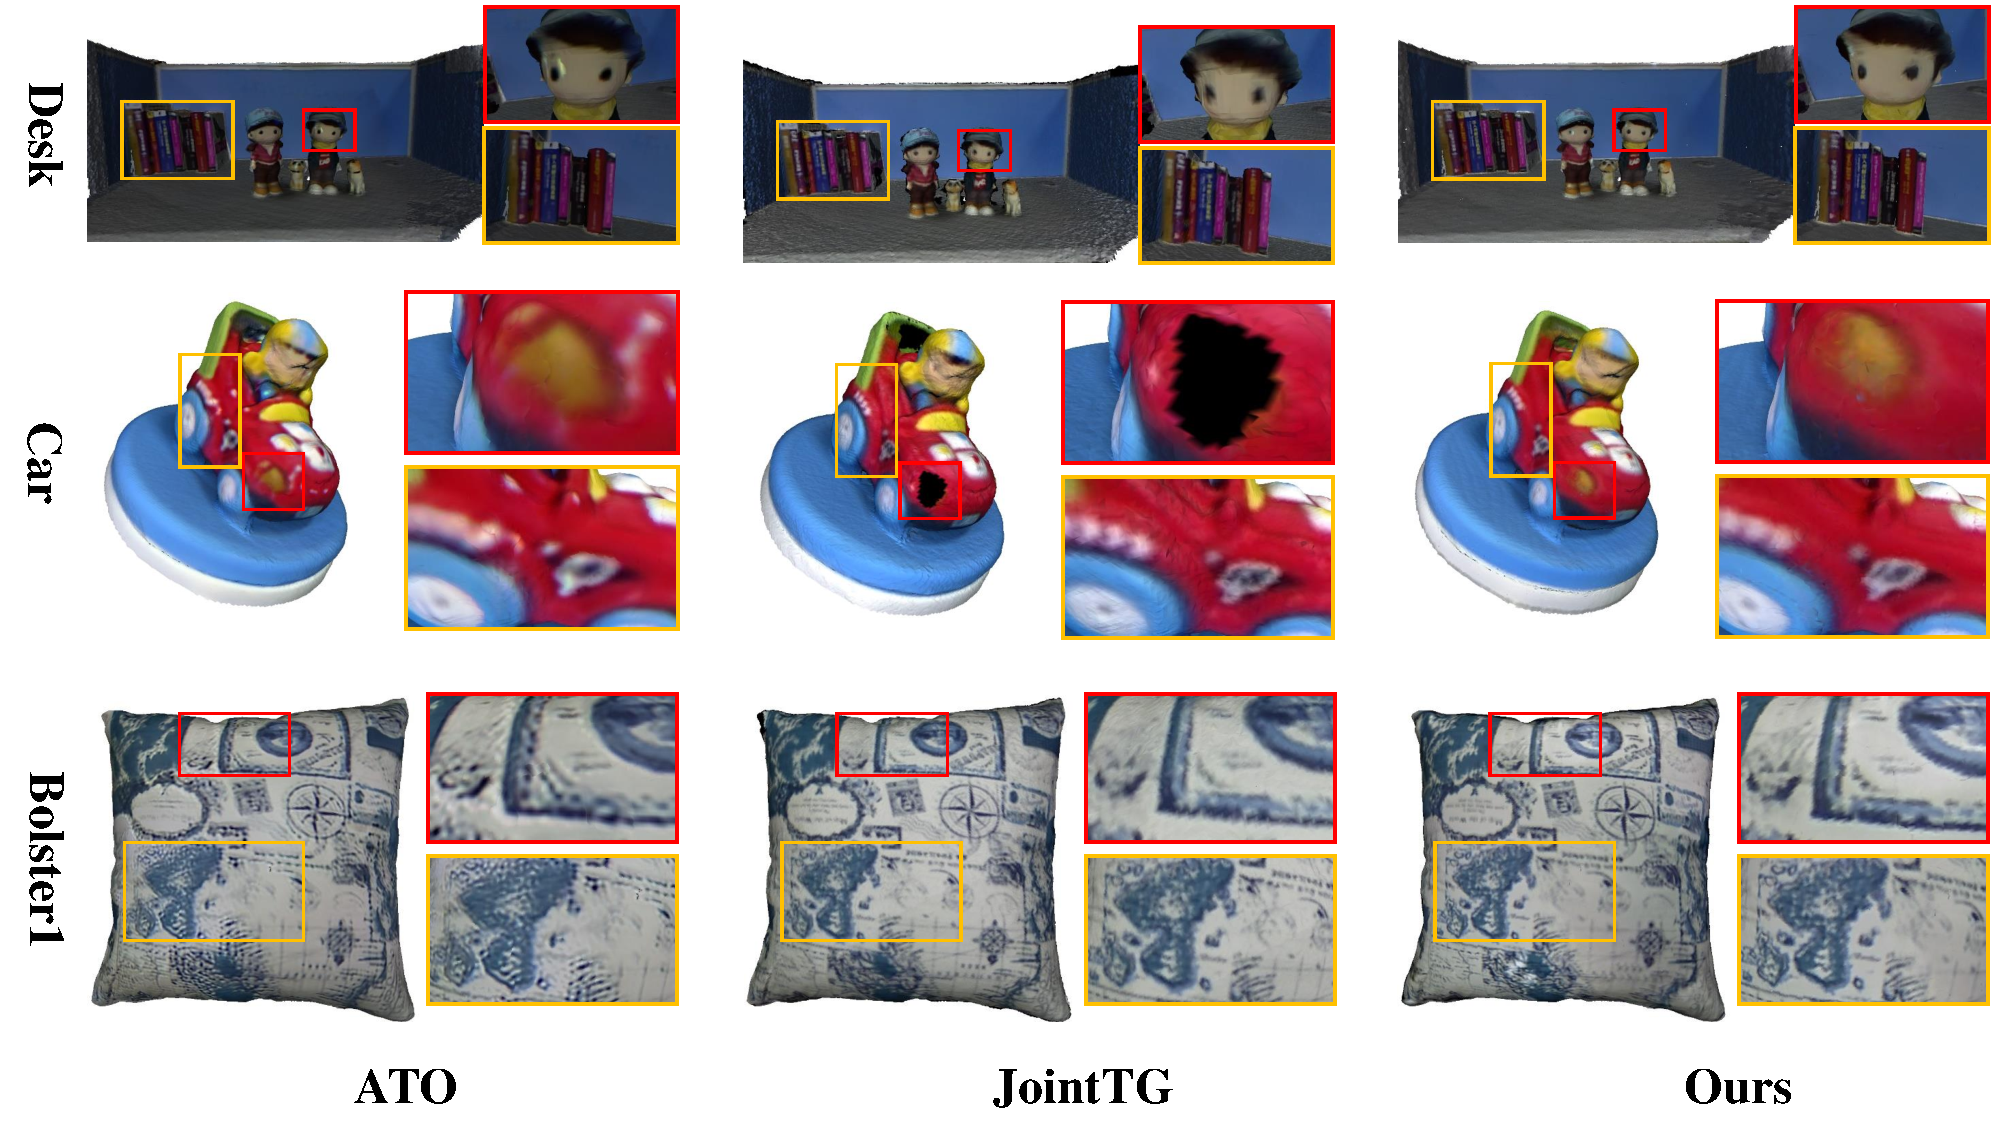
\includegraphics[width=1\linewidth]{pic/work2/compare2.pdf}
\bicaption{公共数据集上不同渲染方法的视觉比较 3}{Visual comparison of different rendering methods on public datasets 3}
\label{fig:ex2_2}
\end{figure}



\subsection{消融实验}
\begin{figure}[!t]
\centering
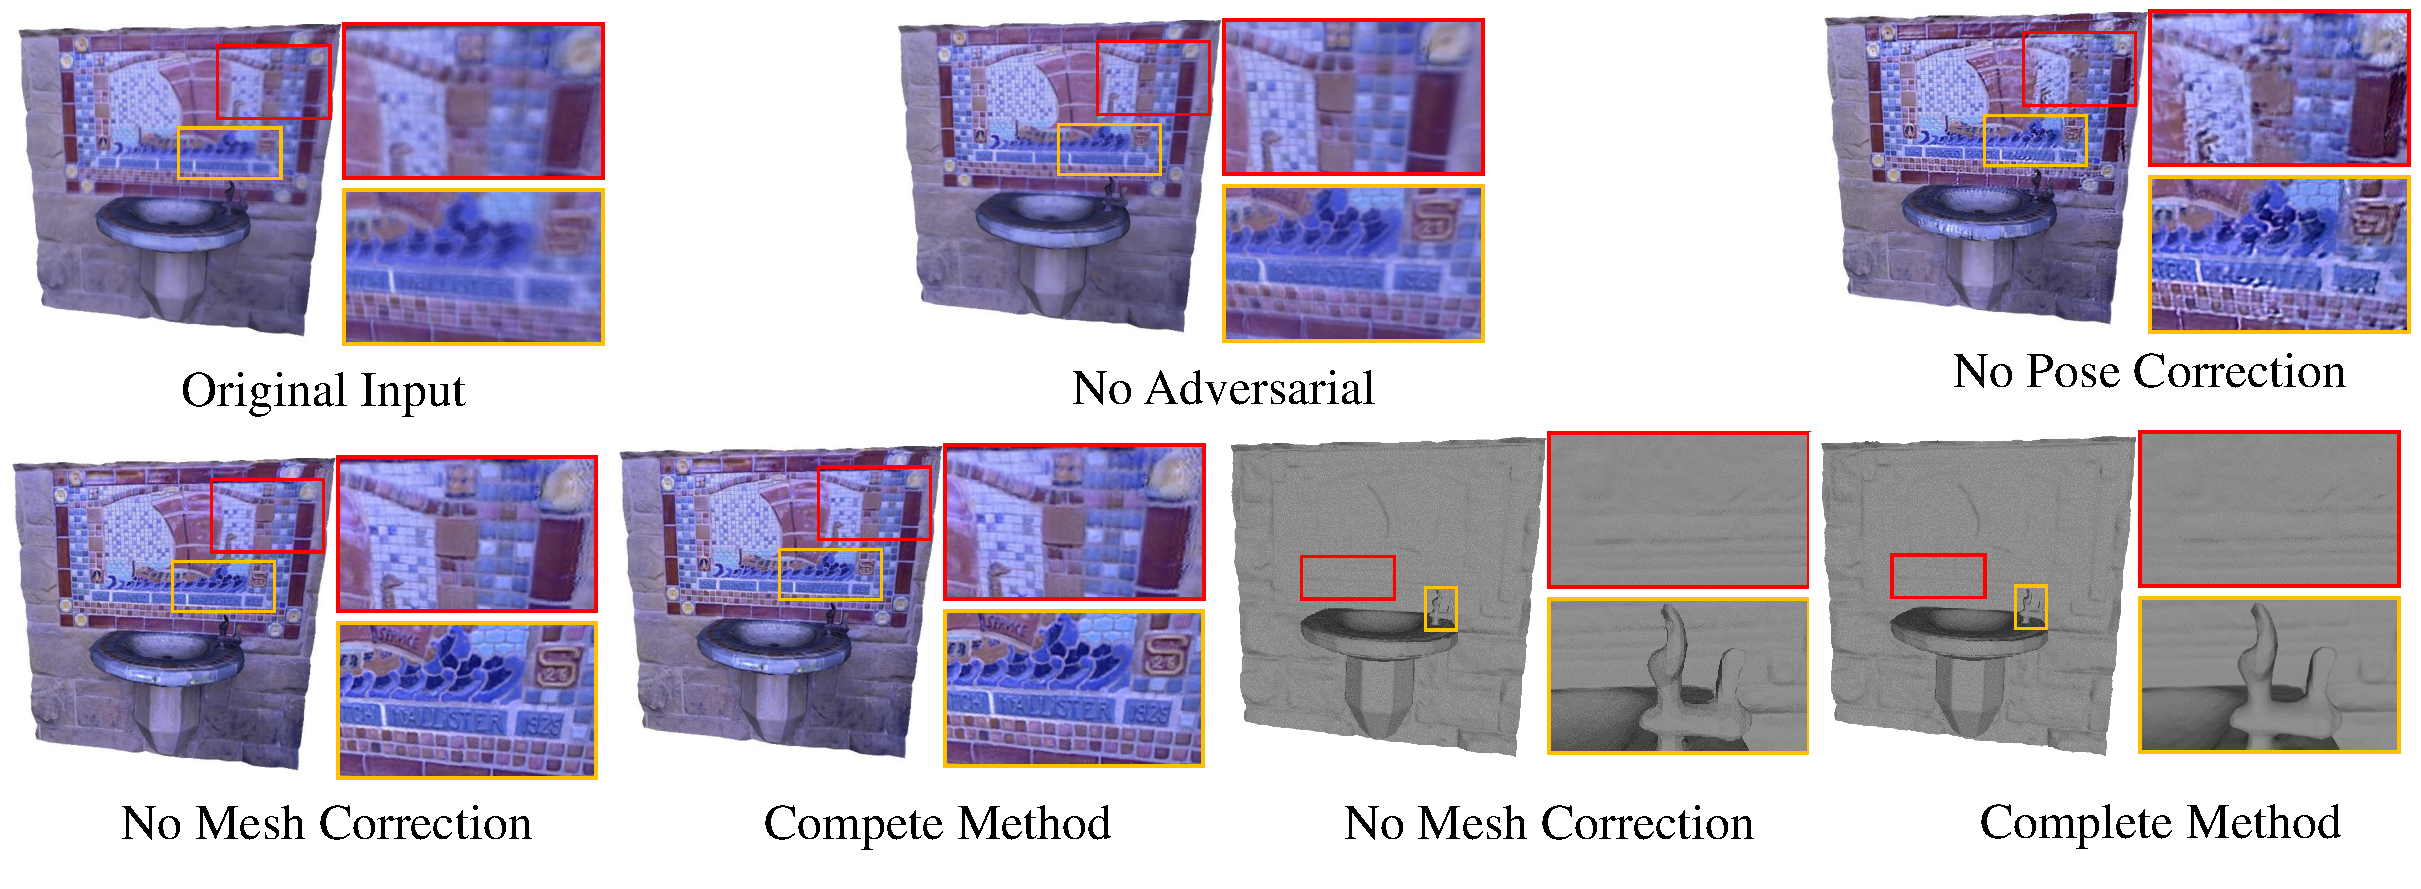
\includegraphics[width=1\linewidth]{pic/work2/compare4.pdf}
\bicaption{消融实验中纹理几何与相机位姿的定性比较}{Qualitative comparison of texture geometry and camera pose in ablation studies}

\label{fig:ex2_5}
\end{figure}





在这个部分,本文研究渲染框架中各个部分的有效性。为了更有说服力,本文选择公共数据集\emph{Fountain}。首先本文在没有矫正相机位姿,没有优化几何模型,没有对抗生成网络的情况下进行实验。最后,本文讨论自适应细分方法中基于面片的细分和基于边的细分区别。\par
如图~\ref{fig:ex2_5}和表~\ref{tab:ablation2}所示,本文展示了移除优化流程中的各个部分效果。没有矫正相机位姿情况下,渲染图片和真实图片会有错位现象,借助于对抗生成本文仍都能得到貌似真实的纹理,但是细节之处会失真。没有几何优化,看起来对纹理生成效果最小,几何误差的影响更多是局部的,因此几何细化不如相机位姿校正重要。本文在图片第二行展示了几何细化的效果。经过几何优化后,模型细节处看起来更加平滑,模型本身的高频几何细节更明细。没有对抗生成网络时,无论是纹理细节还是整体视觉效果都会不同程度的下降。本文消融研究表明,相机姿态、几何形状和纹理相互影响,因此联合优化是必要的。\par

\begin{table}[!h]
\renewcommand{\arraystretch}{1.3}
\bicaption{消融实验中纹理几何与相机位姿的定量比较}{Quantitative comparison of texture geometry and camera pose in ablation studies}
\label{tab:ablation2}
	\centering
%    \scalebox{0.80}{
		\begin{tabular}{lcccc}
			\hline
			{Methods} & \tabincell{c}{No pose \\ correction} & \tabincell{c}{No geometry \\ refinement} & \tabincell{c}{No adversarial \\ loss} & \tabincell{c}{Complete \\ method} \\
			\hline
			PSNR$\uparrow$ & 23.215 & 29.336 & 28.374 & \textbf{30.310}\\
			SSIM$\uparrow$ & 0.810 & 0.844 & 0.864 & \textbf{0.842}\\
			Perceptual$\downarrow$ & 0.094 & 0.067 & 0.055 & \textbf{0.055}\\
			\hline
		\end{tabular}
%	}
%	\normalsize
\end{table}

本文采用自适应细分方法,在纹理丰富处产生更多的顶点,保证视觉效果的同时减少数据量。如图所示,本文分别基于面和基于边的做法,虽然基于边的细分能产生更加均匀的效果,但是会导致未细分面片和已细分面片的公共边上的顶点产生度数不平衡状态,而基于面的做法保持规整。当优化几何模型时,基于边的细分容易导致拓扑结构的破坏,即三角形变形为四边形从而产生奇怪的几何模型。如图~\ref{fig:Triangles}(b)所示,红色圆圈标注的顶点为细分后新增加的顶点,如果该顶点在优化过程中位置发生移动,那么顶点所在边会变为两段折线破坏了三角形的拓扑结构。基于以上原因的考量,本文在自适应细分中采用基于面的质心细分方法。
\begin{figure}[ht]
\centering
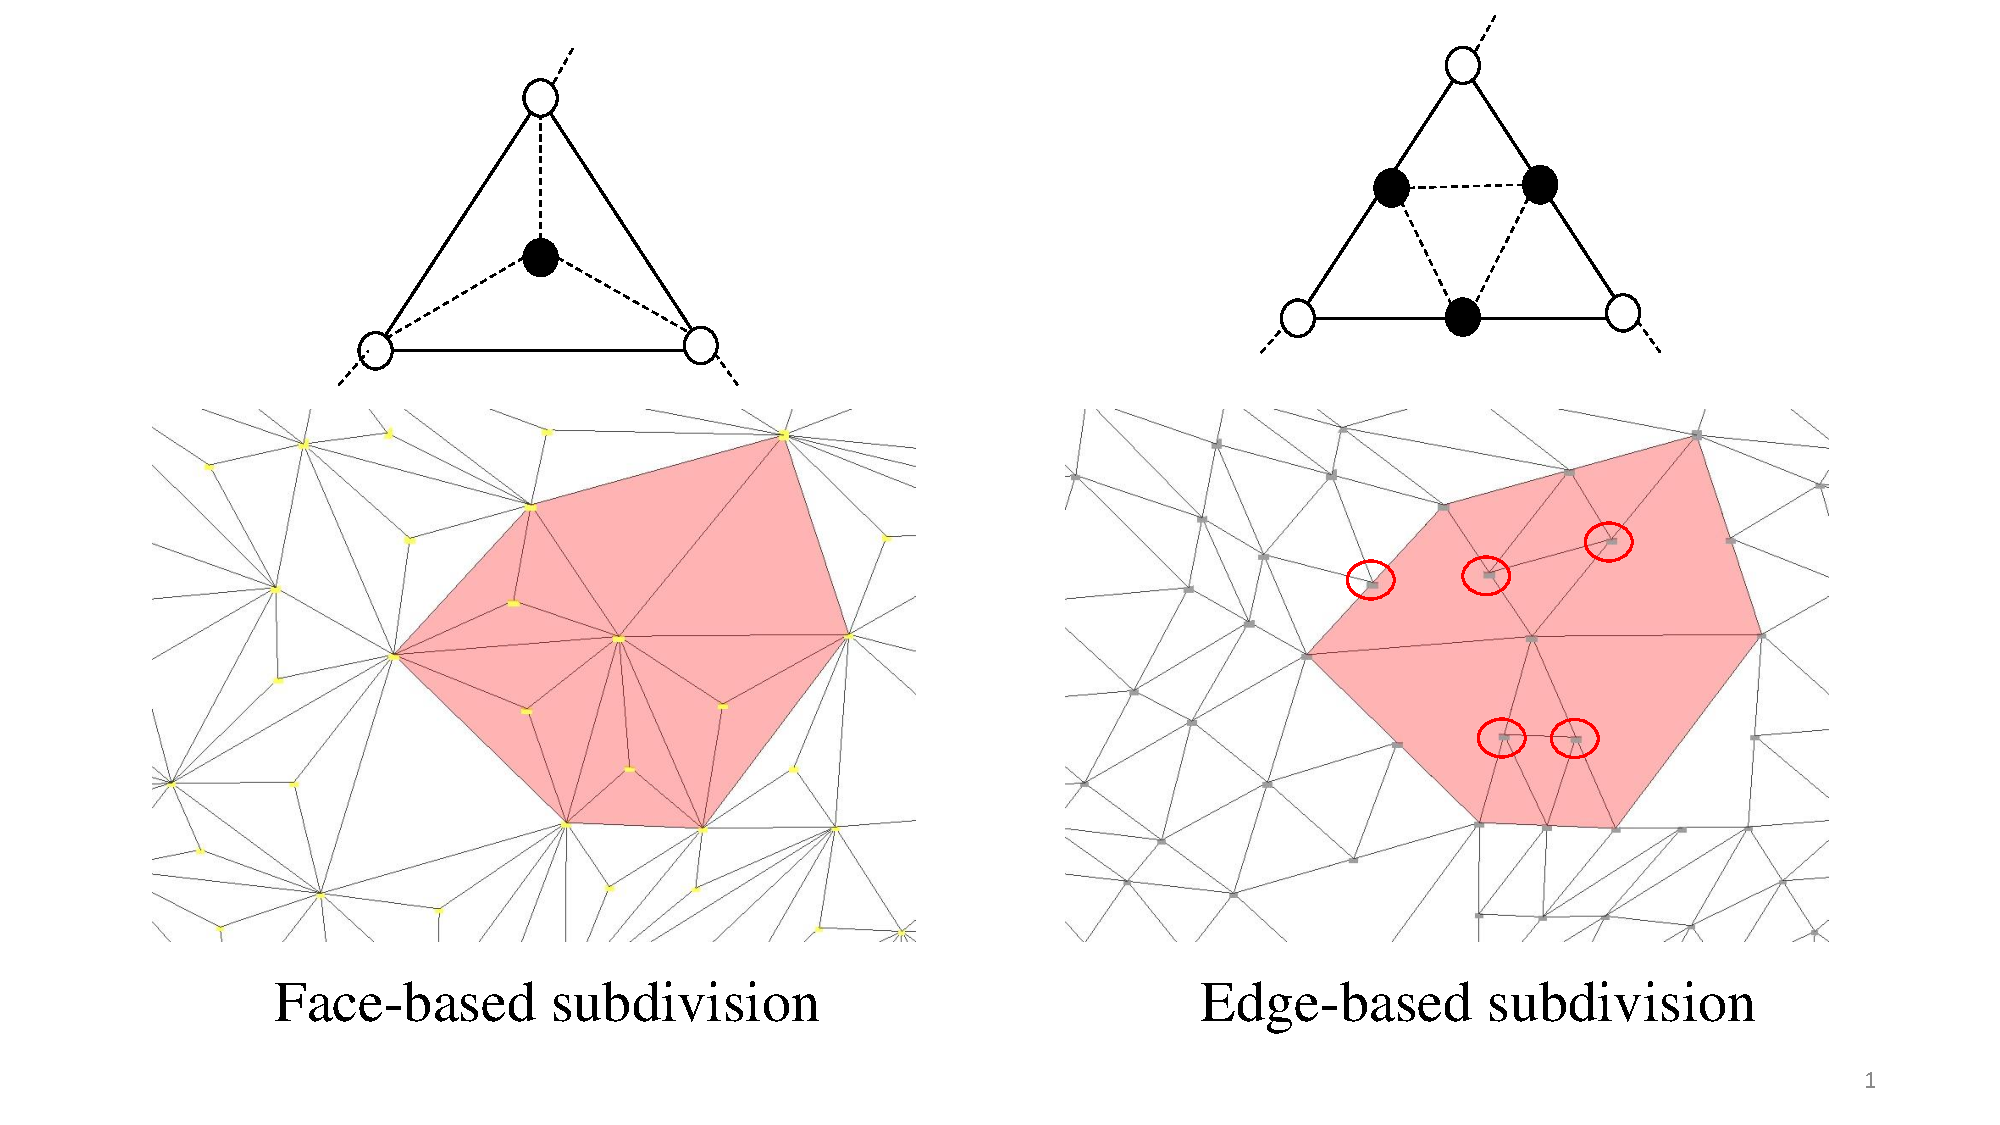
\includegraphics[width=1\linewidth]{pic/work2/Tri.pdf}
\bicaption{基于面和基于边的三角形细分方法的区别}{
Differences between face-based and edge-based triangle subdivision}
\label{fig:Triangles}
\end{figure}
\subsection{算法局限性}
本文采用联合优化方案能够解决三维模型重建误差较大的缺陷取得了一定的效果,但是经过研究发现仍然存在一定的不足。具体地,需要改进的地方如下:\par
\begin{enumerate}[label=(\arabic*),leftmargin=\parindent,align=left,labelwidth=\parindent,labelsep=0pt]
	\item 对于大场景下的纹理优化存在一定的局限性。在大场景下纹理图像需要多张并组合为完整的纹理场景,但是本文无法在优化多张纹理图时保证映射关系,所以本文只关注在单张纹理图可表达的场景。
	\item 无法估计场景光源。在室内点光源以及室外由于反射带来的高光会使被扫描物体表面产生亮点,遮盖了物体表面本身的色彩。优化结果会使物体的漫反射图和高光杂揉到一起无法分离,无法反映物体真实的纹理。 虽然本文能抵抗弱光源带来的误差,但是对于强光源带来的影响无法消除。
	\item 弱纹理场景优化效果不足。本文算法依赖于重投影误差,对于纹理简单的场景,该算法所带来的优化效果并不如纹理丰富的场景那么显著。具体地,无纹理或弱纹理区域,彩色图像上像素值差异不明显,需要利用深度图来协助监督。而且,当场景中弱纹理区域在平面上时,深度差异较小,会进一步减弱算法的监督效果。
\end{enumerate}

\section{本章小结}

本章提出了一种联合优化算法,用于优化RGB-D重建模型的纹理、相机和几何。该算法首先利用重投影误差矫正相机位姿,并应用变形场校正投影像素坐标;随后,利用一致的目标函数更新网格顶点位置,并采用自适应细分来增加网格高频几何细节;最后,本文采用对抗生成网络进行纹理图像重叠,并通过像素重生成管线使像素位置发生位移以抵消重建中的误差。经过联合优化,本文获得了高质量的几何模型、清晰的纹理图像以及精确的相机位姿。实验证明,本文的算法表现出了在各种不同场景下均能重建出高保真度纹理模型的优势。

